\section{Prüfungsvorbereitung: Musterfragen}

\subsection{Frage 1: Was sind Zünfte?}

\textbf{Fragestellung}

Worum handelt es sich bei den Zünften?

\textbf{Antwort}

Zünfte waren Zusammenschlüsse von Handwerkern im Mittelalter und in der Frühen Neuzeit.

Sie regelten:

\begin{itemize}
\item Ausbildung von Lehrlingen
\item Qualitätsstandards
\item wirtschaftliche Interessen
\item Zugang zu bestimmten Berufen
\end{itemize}

Ziel war die Kontrolle handwerklicher Produktion sowie die Sicherung der wirtschaftlichen Stellung ihrer Mitglieder.

\subsection{Frage 2: Weshalb scheiterte Fords Kautschukprojekt im Amazonas?}

\textbf{Fragestellung}

Warum wollte Henry Ford eine eigene Kautschukplantage errichten und weshalb scheiterte das Vorhaben?

\textbf{Antwort}

Ford benötigte grosse Mengen Kautschuk für die Reifenproduktion seiner Automobile. Durch eine eigene Plantage wollte er sich vom internationalen und kolonial geprägten Kautschukhandel unabhängig machen.

Das Projekt scheiterte jedoch aus mehreren Gründen:

\begin{itemize}
\item mangelndes Wissen über tropische Landwirtschaft
\item ungeeignete Managemententscheidungen
\item Krankheiten und Probleme beim Kautschukanbau
\item Widerstand der lokalen Bevölkerung gegen die vorgegebenen Arbeits- und Lebensweisen
\end{itemize}

Das Beispiel zeigt die Grenzen technischer und wirtschaftlicher Planung in fremden ökologischen und sozialen Kontexten.

\subsection{Frage 3: Warum wurde Umwelt in den 1970er Jahren zum Politikum?}

\textbf{Fragestellung}

Welche Faktoren führten dazu, dass Umweltfragen in den 1970er Jahren politisch wichtig wurden?

\textbf{Antwort}

Seit den 1960er und 1970er Jahren wurden Umweltprobleme zunehmend öffentlich wahrgenommen.

Wichtige Gründe waren:

\begin{itemize}
\item Berichte über Umweltkatastrophen
\item Fernsehreportagen und Medienberichte
\item populärwissenschaftliche Veröffentlichungen
\item wissenschaftliche Forschung zu Umweltproblemen
\item Entstehung von Umweltbewegungen
\item Proteste gegen technische Grossprojekte wie Kernkraftwerke
\end{itemize}

Dadurch entwickelte sich Umwelt von einem wissenschaftlichen Thema zu einer gesellschaftlichen und politischen Frage.

\subsection{Frage 4: Quellenkritik zur Frankfurter Küche}

\begin{center}
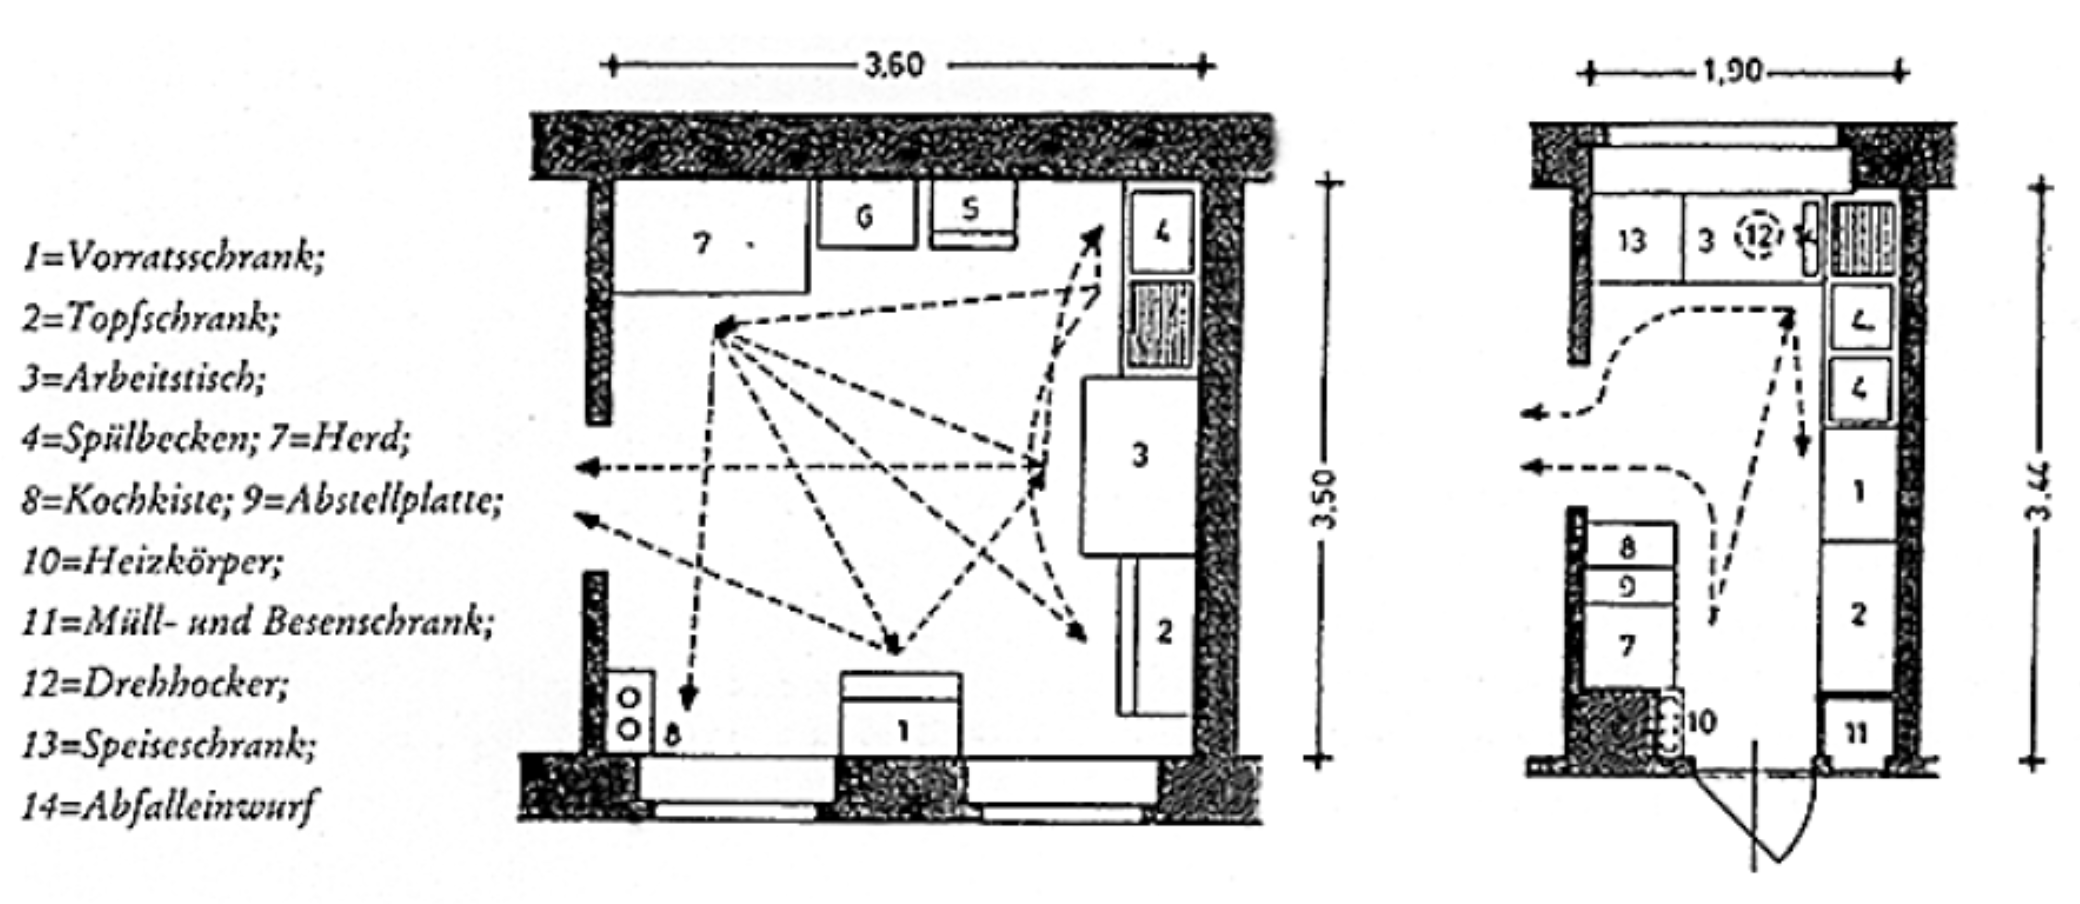
\includegraphics[width=0.8\linewidth]{images/frankfurter_kueche.png}
\end{center}

\textbf{Fragestellung}

Beschreibe Aufbau und Gestaltung der Küche, erläutere die Rationalisierungsprinzipien und interpretiere die Quelle im Hinblick auf moderne Haushaltsführung.

\textbf{Antwort}

Die Frankfurter Küche wurde in den 1920er Jahren entwickelt und sollte Hausarbeit effizienter gestalten.

Herd, Spüle, Arbeitsflächen und Schränke sind so angeordnet, dass Arbeitswege möglichst kurz bleiben. Die Küche ist kompakt, funktional und stark standardisiert.

Die Gestaltung orientiert sich am Scientific Management von Frederick Taylor. Arbeitsabläufe werden analysiert und optimiert, um Zeit und Kraftaufwand zu sparen. Damit werden industrielle Rationalisierungsprinzipien auf den privaten Haushalt übertragen.

Die Quelle zeigt moderne Vorstellungen von Ordnung, Hygiene und Effizienz. Gleichzeitig macht sie deutlich, dass Hausarbeit weiterhin überwiegend Frauen zugewiesen wurde. Die Frankfurter Küche steht daher sowohl für technischen Fortschritt als auch für Standardisierung und Disziplinierung des Alltags.

\subsection{Zentrale Erkenntnisse}

Für die Prüfung besonders wichtig:

\begin{itemize}
\item Zünfte regulierten handwerkliche Arbeit und Ausbildung.
\item Ford wollte Rohstoffe kontrollieren, scheiterte aber an lokalen Bedingungen.
\item Umwelt wurde durch Medien, Wissenschaft und soziale Bewegungen politisiert.
\item Die Frankfurter Küche übertrug industrielle Rationalisierung auf den Haushalt.
\item Technikgeschichte untersucht immer auch soziale, politische und kulturelle Folgen technischer Entwicklungen.
\end{itemize}
